\chapter{Literature Review}
\label{ch:background}

In this chapter, we present previous works that investigated the effect of 
computational environments on scientific results:
showing the magnitude of the effect of computing environment changes such 
as hardware and software implementations. Next, we review 
techniques and tools to enhance the reproducibility of experiments 
including code and data sharing methods using version control 
systems, and virtualization techniques to encapsulate computational 
variability of the analysis. 
% We presents the role that numerical stability plays in these problems 
% several case studies in neuroimaging to demonstrate the necessity of
% exploring numerical stability in this space.
Finally, we describe provenance management tools
to collect and represent the analysis dependencies. 


\section{Computational Reproducibility}

Many works have investigated the reproducibility of computational
pipelines in the past few years. In general, analysis results are not reproducible
because of the numerical errors caused by computing environment changes,
including hardware configuration or operating system. 

Changes in the computational conditions may introduce small numerical 
errors, subsequently propagated and amplified by pipelines.
The analysis pipelines are said to be numerically unstable. 
Numerical instability is a characteristic of the pipelines which 
amplify small numerical errors and then hamper the reproducibility 
of the analyses depending on the complexity of the pipeline and magnitude 
of the errors. In many cases, numerical instability is an important 
issue for reproducibility. 

The following sections discuss the effect of influential elements on 
reproducibility, in particular workstation type, parallelization techniques, 
operating system changes, analysis software variety, and perturbations 
applied in input data. 

\subsection{Effect of Hardware Resources}

The hardware configuration of computers is an 
influential source of irreproducibility~\cite{hill2017numerical}. 
The numerical errors are particularly noticeable across computing processors 
such as CPUs (Central Processing Units), GPUs (Graphics Processing 
Units) and APUs (Accelerated Processing Units), mainly due to incompatibilities 
of floating-point units (FPU) with the IEEE-754 standard when 
arithmetic precision of the floating-point values are not specified 
uniformly.

Even using the same arithmetic precision, it is difficult to achieve 
bitwise identical results across different hardware resources. 
Recent studies show that hardware developments to improve 
computational performance sacrifice numerical 
reproducibility~\cite{duben2014use, demmel2013numerical}. For instance, 
code optimization techniques embedded inside CPUs, known as 
out-of-order execution (dynamic scheduling), impede 
reproducibility because processors might execute 
instructions out of the original order in which they appear based on the 
availability of input data and execution units to use resources 
efficiently~\cite{wiki2018out-of-order}. Therefore, they might compute 
floating-point operations in different order,
which often leads to different results
due to different rounding of the intermediate floating-point arithmetics.
Also, this has been shown in several papers~\cite{duben2014use, demmel2013numerical} 
that some operations in particular sum and division are not associative.

A study~\cite{jezequel2015estimation} implemented
acoustic wave equation to see the effect of processor architecture on 
results. The authors illustrate irreproducible results across 
different processors including AMD CPU, NVIDIA GPU, and AMD APU, even 
using the IEEE-754 standard. The results numerically vary from one 
architecture to another, the maximal relative difference between 
results in the range [0.1, 1] and its mean value is $10^{-5}$. Such 
differences often occur due to rounding errors generated by different 
orders in the sequence of arithmetic operations.

In neuroimaging, it is important to evaluate the consistency of  
results when they are executed on heterogeneous computing systems
that use more than one kind of processor or core.
A number of tests were conducted 
~\cite{Gronenschild2012} to gain insight into the variability of  
results from neuroimaging packages based on different data processing 
conditions like different workstation types. Two
different types of workstations were compared: an HP (Hewlett Packard) one 
using Centos 5.3 and 8 CPU cores, and a Mac one using OSX 10.5.8 and 2 
CPU cores. This study showed significant absolute differences among 
the volumes of anatomical structures obtained on the two different 
workstations. 
These differences were on average 8.8±6.6\% (range 1.3–64.0\%) (volume) and 2.8±1.3\% (1.1–7.7\%) (cortical thickness). 


\subsection{Effect of Parallelization}

Developers leverage parallelization techniques to accelerate the 
execution performance at different levels, from multi-threaded programming to 
high-performance computing (HPC). With parallelization techniques, contrary to 
sequential implementations, the execution order of the processes may 
change in different runs. Consequently, several runs of the 
parallelized code may produce different 
results, even on the same computer. 

To show the existence of such issues, the impact of the number of 
processors on numerical reproducibility was studied 
~\cite{diethelm2012limits}. This study simulated the process of 
deformation of metal sheets in the packaging industry to measure local 
change of the sheet thickness using different number of processors. 
Results obtained significant differences in maximal and minimal values of sheet thickness changes
originating from the nondeterministic behavior of a program code linked
to a component of \href{http://software.intel.com/en-us/intel-mkl}{the Intel Math Kernel Library}.
Their findings showed the amplification of rounding errors in summations after running the same 
simulation on the same computers with a different number of processors. 
This also proved that the summation operation is not associative because of 
different rounding of the intermediate floating-point results, even 
using the standard IEEE double-precision arithmetics. Therefore, final 
result of the summation depends on the order in which values are 
processed, which changed by the number of processors. 

Another statistical simulation showed reproducibility failures in 
multi-core processing performed on GP-GPUs and multi-core 
CPUs~\cite{taufer2010improving}. Multi-core architectures enable 
multi-threaded environments for running numerical intensive applications 
at high speeds. This study showed that the stability of molecular 
dynamics simulation results is not guaranteed in multi-core processors 
due to different orders of floating-point operations (e.g., 
division and square root operations) leading
to different rounding and truncation. 

In addition, parallel programming may lead to vulnerabilities like race conditions that 
further impede reproducibility. A race condition is a situation in 
concurrent programming where two concurrent threads or processes have 
access to the same resources and attempt to change it at the same time. 
When one thread is performing read on a particular data element, 
another thread is allowed to modify or delete this element. The 
resulting final state depends on the order of the operations, which 
is not correctly programmed by the application developers. In addition to race condition, 
some other problems have been listed as the main sources of numerical 
differences in many parallelized experiments such as out-of-order 
execution, and message buffering non-blocking communication 
operations~\cite{revol2014numerical}. 

Message buffering is a type of communication using send/receive 
functions in parallel programming, which can be blocking and 
non-blocking. 
Non-blocking communication means that computing and transferring data can happen at 
the same time for a single process. This allows communication to 
overlap, which generally can speed up the process but also can lead to different computing orders and 
irreproducible results for different runs. 

Furthermore, some experiments~\cite{Gronenschild2012} 
determined the effect of parallelization on neuroimaging pipelines, 
most precisely in different versions of FreeSurfer. 
They showed that concurrent running would not make 
statistically significant differences based on the comparison of voxel 
volume of specific brain structures for the same conditions. This is an 
example where Peng's reproducibility is achieved while numerical 
reproducibility is not.
However, further experiments are needed to investigate the effect of parallelization on neuroimaging.

\subsection{Effect of Operating Systems}

We summarize results~\cite{Glatard2015}
that quantified the reproducibility of computational analyses 
across operating systems. In particular, the authors determined 
the reproducibility of three neuroimaging workflow packages, FSL, 
FreeSurfer, and CIVET between CentOS 5.10 and Fedora 20. 

Using FSL, cortical and subcortical tissue classifications resulted in
Dice values as low as 0.59 between the classified tissues on CentOS 
and Fedora operating systems. These differences mainly correspond to 
the mathematical functions implemented in different operating system 
libraries. 

The results of \emph{RS-fMRI} analysis revealed significant inter-OS 
differences in the second experiment, which showed that each 
pre-processing step could introduce small numerical variations ans that their 
accumulation creates important differences. These numerical differences 
are caused by changes in the implementation of mathematical functions like 
\emph{sinf()} between operating systems.  

Using FreeSurfer and CIVET, cortical thickness extractions
had important differences in some specific brain regions across 
operating systems. Figure~\ref{inter_os} shows localized regions of 
these differences for CIVET, which are quantified by
mean absolute difference, standard deviation of absolute 
difference, t-statistic and random field theory (RFT). 
Areas in shades of blue on the RFT map are significant at the cluster level.

Additionally, inter-build differences are measured in this study. A 
static build of a pipeline refers to its compiled version where 
libraries are statically linked. The authors used the 
static builds of FreeSurfer CentOS 4 and CentOS 6 to measure their 
reproducibility. Results of FreeSurfer show that building static programs improves 
reproducibility across OSes, but small differences still remain
(the t-statistic values of $±2$). The 
main cause of such differences is dynamic libraries that are loaded by 
the static executable at run-time. 

\begin{figure}[H]
\centering
	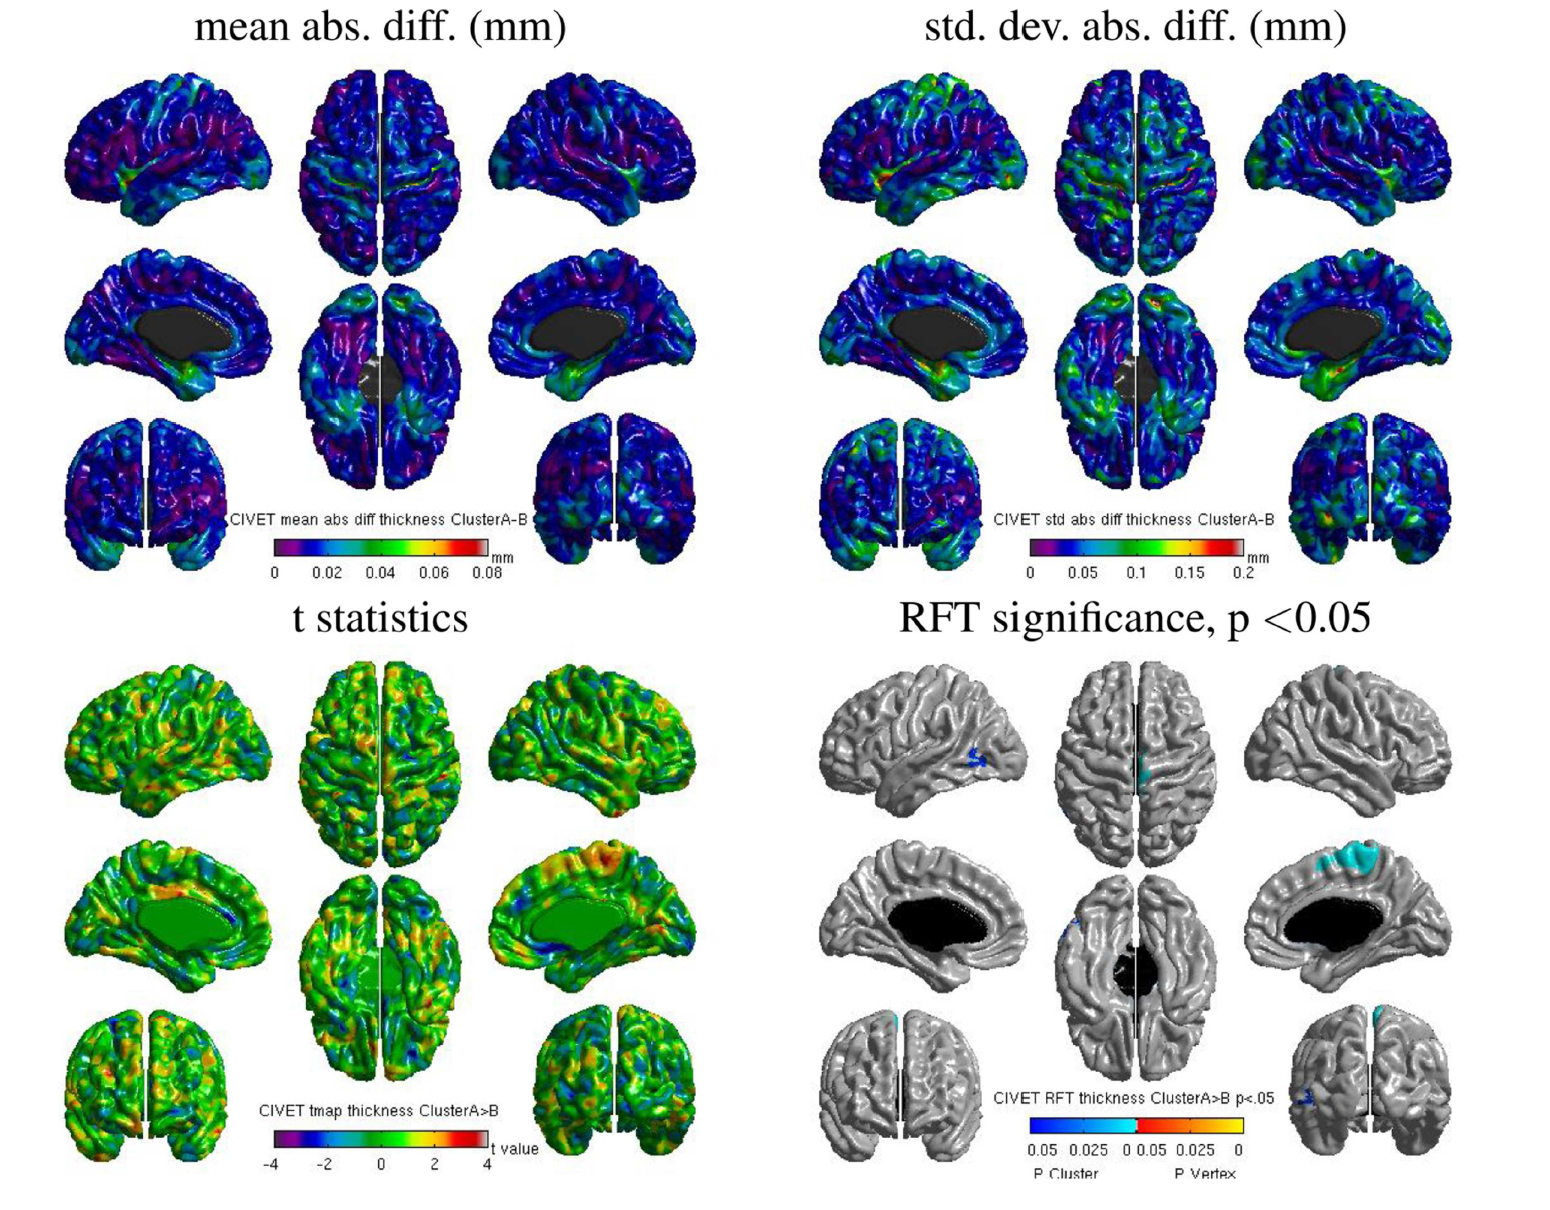
\includegraphics[scale=0.9]{chapters/background/images/inter-os-diff} 
	\caption{Surface maps of four metrics, standard-deviation and mean 
	absolute differences, t-statistic and RFT significance values, 
	indicate the inter-OS differences for the cortical thickness 
	extracted with CIVET over 146 subjects~\cite{Glatard2015}. } 
	\label{inter_os}
\end{figure}
 

The work~\cite{Glatard2015} detected that most of
neuroimaging pipelines are sensitive to operating 
systems. The effect size of the variations is changed based on the 
complexity of the analysis pipeline. For instance, shorter analyses 
like brain extraction have much less significant disagreement compared 
to longer ones like subcortical tissue classification and RSfMRI
analysis because of the accumulation of numerical errors in the complex analyses.

Furthermore, in future works, the authors expect similar reproducibility issues for the 
other Linux distributions including Debian and Ubuntu as long as they 
are based on glibc, the GNU C library, which includes mathematical 
libraries. Other studies~\cite{Gronenschild2012, 
Krefting2011} reported similar issues for non-Linux operating systems. 


\subsection{Effect of Analysis Software}

Reproducibility of computations also depends on the executed analysis 
software, even using the same operating system and hardware resources. 
Different version of an analysis software used in a computation may 
produce different results. Also, the re-implementation of the same 
experiment through different software packages can introduce 
discrepancies between their results. We summarize the impact of 
software variability including different software versions and a wider 
range of software packages on reproducibility of results. 

\subsubsection{Effect of software versions} 

In addition to comparing hardware and operating system variability,
~\cite{Gronenschild2012} studied the impact of using different pipeline 
versions.
Significant volume differences are quantified across the FreeSurfer 
versions for both anatomical brain structures and cortical thickness 
measures. 

The same study~\cite{Gronenschild2012} showed that the effect 
sizes of different operating systems or software versions are close to 
the ones measured in neuropsychiatric diseases. For example, the impact 
of Alzheimer disease and semantic dementia on grey matter volume changes
% are reported in~\cite{lehmann2010atrophy}. These results
show similar changes between volumes of specific structures compared to 
the discrepancies caused by computation environment variability 
~\cite{Gronenschild2012}. In addition, differences in cortical 
thickness caused by various operating systems, software versions and 
workstation types were roughly of the same order of magnitude than 
findings~\cite{kuperberg2003regionally} from patients who 
suffered from schizophrenia. There are many other proofs in different 
domains that show the influence of software updates on  
results~\cite{shim2015effect, wadi2016impact}.

\subsubsection{Effect of software packages} 
\label{swf_effect}

In all aforementioned analyses, the choice of the software package 
remained fixed for carrying out the analyses in each study. To understand 
out the impact of analysis software variations on task fMRI results, 
several tests were conducted~\cite{bowring2019exploring}. The authors 
investigated differences produced across three of the most popular 
neuroimaging software packages, AFNI, FSL, and SPM. They replicated 
specific analyses, a number of image processing steps, as closely 
matched to the original study as possible. 

The statistical comparisons show a substantial disagreement between 
software package results, producing different location of 
activation regions. 
Figure~\ref{inter_sfw} shows the substantial variation 
between each main activation area found in the original study and the 
reanalyses. Results indicate that the precise location of the significantly 
activated regions is highly dependent on the choice of software package 
and inference method.

\begin{figure}[H]
\centering
	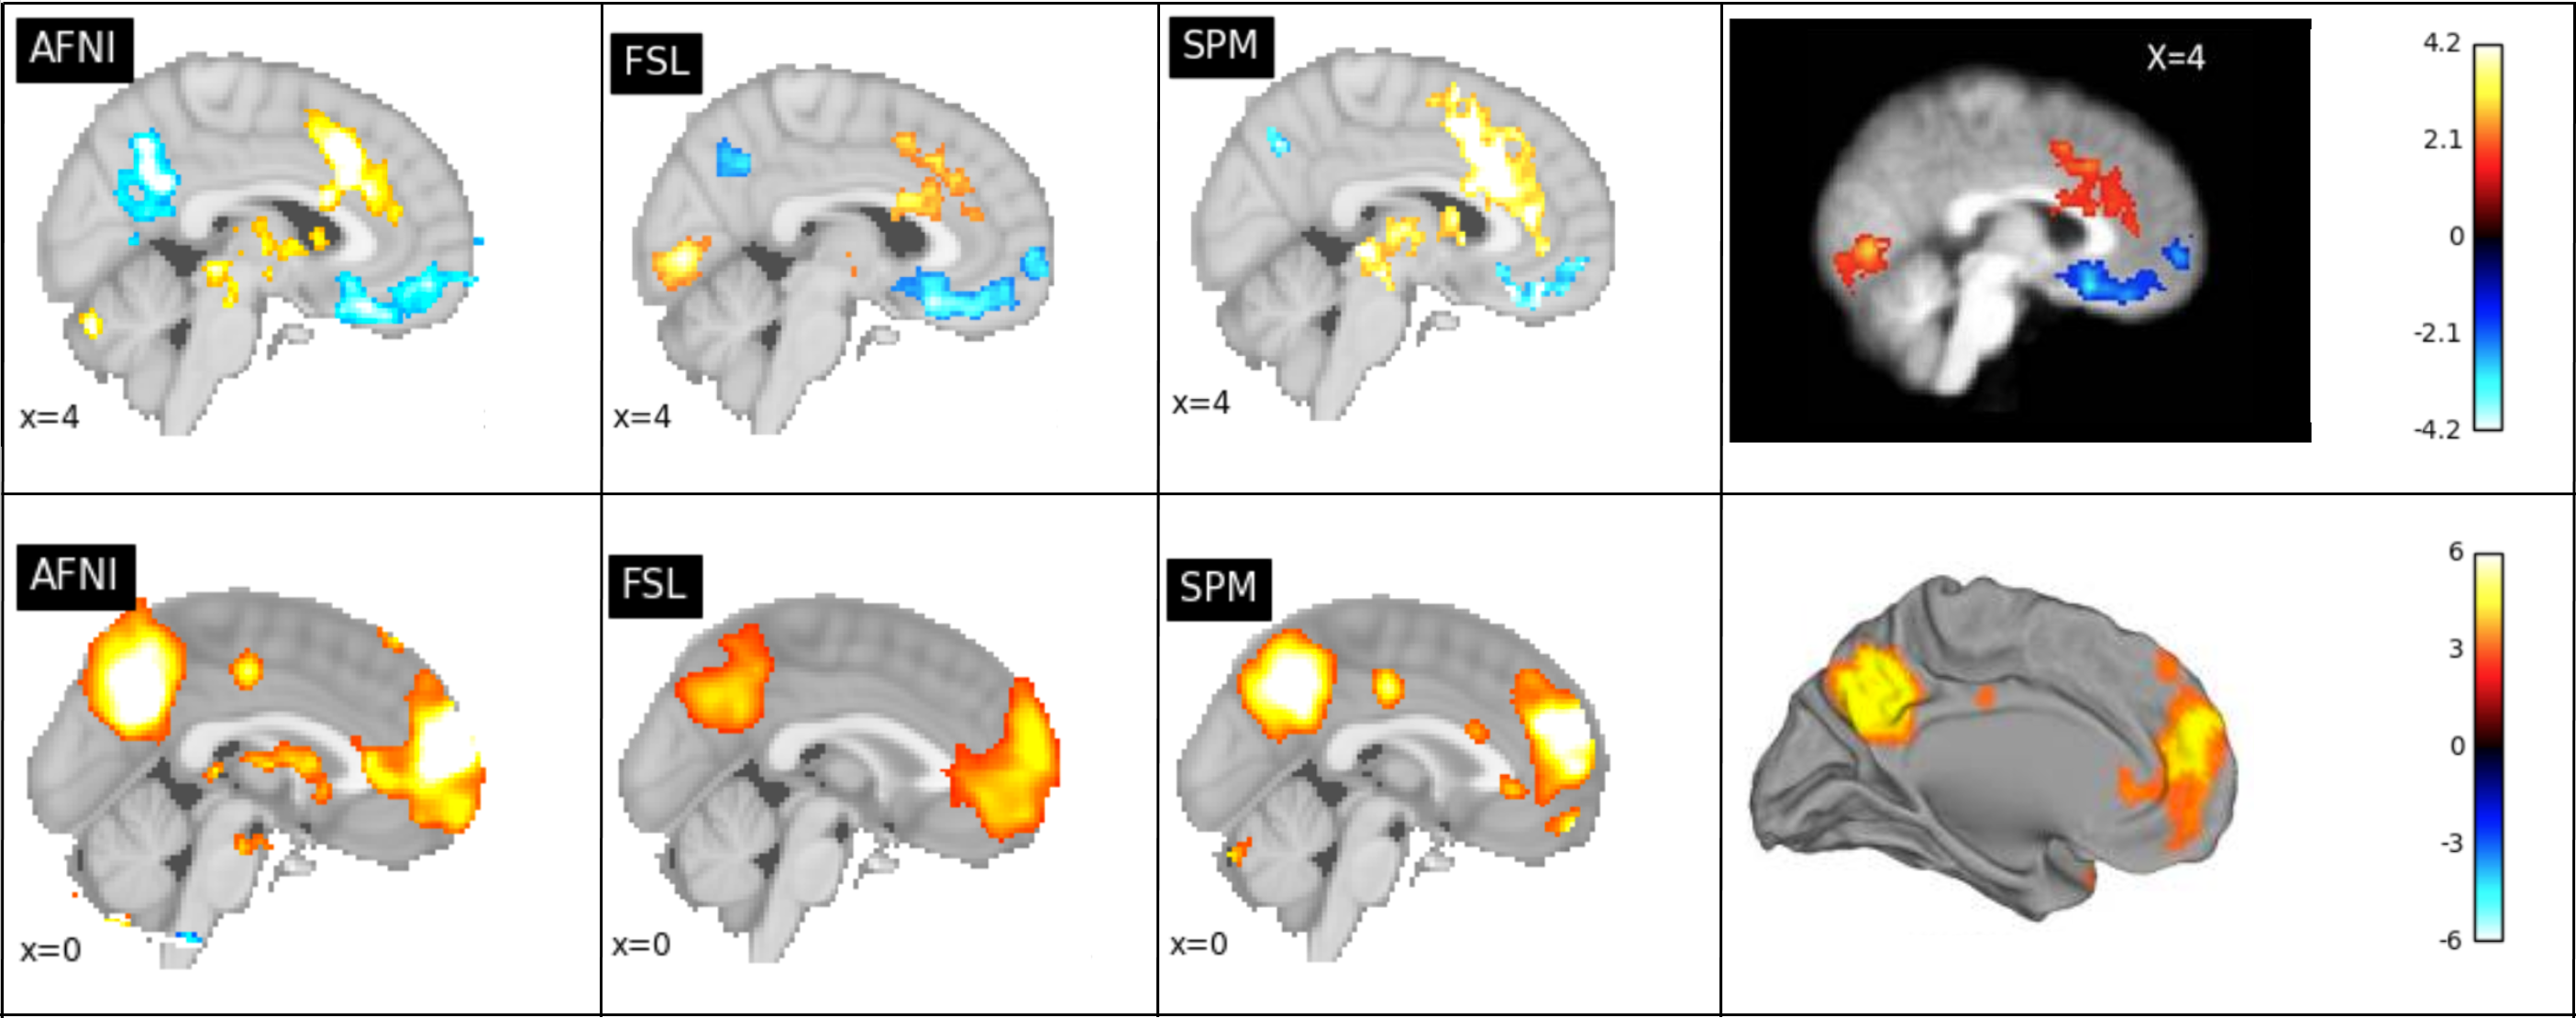
\includegraphics[scale=0.5]{chapters/background/images/inter_sfw} 
	\caption{Comparison of the thresholded statistic maps of two 
	different analyses within AFNI, FSL and SPM. Each row shows the 
	results of each reanalyses, and the last column shows the main 
	figure from the original publication. Total 16 subjects and 21 
	subjects are participated in the first study (first row) and second 
	study (second row) respectively~\cite{bowring2019exploring}.
	\label{inter_sfw}}
\end{figure}

Analyses~\cite{bowring2019exploring} found that the size of datasets 
can contribute to the variation of results. For instance, results 
obtained from analyses that use smaller sample size are less likely to 
be reproducible than analyses in which more subjects participated.
This is likely explained by the fact that group analyses benefit from
regularization of numerical noise, which is expected to increase with sample size. 
Therefore, variation in the outcome of an fMRI analysis depends not 
only on the choice of software package used, but also on the dataset 
being analyzed. 

\subsection{Effect of Small Data Perturbations}

Neuroimaging pipelines 
are sensitive to changes in the computing environment. 
Studies were conducted to show the instability of some specific 
steps of MRI analysis through the simulation of minor perturbations in 
input data. For instance, reproducibility of the cortical surface 
reconstruction analysis in the presence of small perturbations is 
measured in~\cite{Lindsay2017hbm}. The authors investigated results of two 
pipelines, CIVET and FreeSurfer, after applying 1\% intensity 
modification on one voxel located in a non-cortical region. Contrary to 
expectations, widespread surface changes were observed across the 
cortex. 

Similarly, another study~\cite{Glatard2018hbm} observed substantial 
variability of motion correction algorithms in fMRI analyses by 
applying one-voxel perturbation. Results demonstrate significant 
differences for Niak and FSL. These 
variations may result in wrong activation maps and increase the 
prevalence of false activations on the subsequent steps of fMRI 
processing. 

Recently, the processing of high-resolution images has been made possible 
through a new version of pipelines.
~\cite{Lindsay2018hbm} quantifies the variability of analysis results 
across different image resolutions. The authors investigated the 
partial volume effects\footnote{Defined as the loss of contrast between two adjacent tissues in an image
because of the limited resolution of the imaging system} of various image resolutions on the automated 
cortical surface extraction through CIVET and FreeSurfer pipelines. 
They shows significant variability in results for the same 
analysis using images with different resolutions. For both pipelines, 
mean absolute error, signed error, and standard deviation are mostly 
reduced as a function of increasing resolution. Also, comparison of 
projected distance error maps between histological ground truth 
surfaces and MRI-derived surfaces confirms that the accuracy of 
analysis is increased in higher resolutions. Further research is needed 
to minimize partial volume effects along with magnifying the resolution 
to get more accurate results. 

% \subsection{Conclusion}

% We reviewed reproducibility of the computational analyses across data 
% perturbations and different computing environments such as operating 
% system, workstation type, software version, etc. We found that these 
% elements have significant effects so that would change the results of 
% analyses. So, reproducibility of analysis is highly dependent on 
% computational environments. Also, it should be noted that the influence 
% of all these elements are of the same importance and each of them 
% cannot be more important than other one. 

% We investigate reproducibility of analyses across small perturbations. 
% Therefore, the choice of analysis software remained fixed to assess the 
% reproducibility issues across a number of computational parameters in 
% my research. In this way, we can determine reproducibility issues 
% caused by the pipeline instability. Accordingly, we will introduce 
% several solutions to address such reproducibility issues in the next 
% chapter. 

\section{Techniques to Improve Reproducibility}
\label{techniques}

Reproducibility is mainly ensured through three properties: 
source sharing for both code and data, 
research portability, and pipeline 
stability. Source sharing and research portability can be related to 
the FAIR principles~\cite{wilkinson2016fair} according to which 
scientific sources have to be findable, accessible, interoperable, and 
re-usable. 

The first step in reproducibility is finding and accessing research products
related to Findable and Accessible principles in FAIR.
Code and data must be publicly available in a 
machine-readable structure. 
It enables the verification of scientific 
results by independent investigators. 

Analysis pipelines must
integrate with other execution environments. This is termed research 
portability and can be achieved using virtual machines and 
containerization technologies. Portability enables researchers to 
re-run analyses in a variety of execution conditions. This can be 
matched with the Interoperability and Re-usability of FAIR principles. 

Analysis pipelines must be numerically stable across
computing environments to be reproducible. Although 
many solutions currently exist to address analysis sharing and 
portability, the effect of numerical instability remains largely 
unexplained. We discuss a number of techniques 
and tools used to enhance sharing, portability, and stability of the 
analyses.


\subsection{Code and Data Sharing}

To successfully reproduce a computational experiment, analysis sources 
must be accessible in a machine-readable 
structure~\cite{stodden2016enhancing,hasham2018cloud}. The importance 
of a proper structure is clear, specifically when we aim to share 
code with others or contribute to a wider group.

One foundation of code sharing is modern software engineering, which 
includes practices like version control systems (VCS). Version control 
ensures that the history of the code is available and archived. 
Git~\cite{git}, as one of the most popular VCS frameworks, provides a 
distributed means to manage project files. Git facilitates the 
collaboration of developers on the same project using GitHub. GitHub is 
a Web-based service for Git, which hosts Git repositories. 

Developers may share programs instead of source code 
because of commercial reasons, simplifying its usage, reproducibility improvement, 
etc. Several sharing tools exist to maintain a set 
of packages. PyPI (Python 
Package Index) is a software repository for the Python programming 
language. PyPI helps to share python packages and allows users to 
search for packages by keywords. There are more specific 
sharing tools for neuroimaging programs including 
Boutiques~\cite{glatard2018boutiques}, a system to publish and 
integrate command-line applications automatically using a JSON 
descriptor, or 
NITRC-CE~\cite{kennedy2016nitrc}, which provides a number of 
pre-installed neuroimaging tools such as AFNI, FSL, and FreeSurfer into 
a standardized computational environment. 

However, there are some challenges 
associated with data sharing including concerns about the privacy of 
personal information, lack of incentive for researchers, and 
technical issues associated with sharing of large datasets. 

Git is a very efficient tool for managing textual information such as 
code, text, and configuration, but it is inefficient for storing large 
data. Therefore, extensions of Git, like git-annex~\cite{git-annex} 
and Git-LFS (Large File Storage)~\cite{git-lfs} were developed to 
address the problem of sharing and versioning large data collections. 
git-annex uses Git to store and index files without committing large 
files into the Git repository. Similarly, Git-LFS reduces the impact of 
file size in the repository by replacing large files with lightweight 
pointer files, which refer to the actual file location. 

Both Git and git-annex allow collaboration on a single 
repository, but sharing code and data between multiple projects can be an 
issue. Also, they lack advanced meta-data search 
capabilities. For instance, they cannot crawl through domain-specific repositories.
Datalad~\cite{datalad} is an 
efficient tool for data sharing and versioning 
multiple datasets. This tool is built on top of git-annex and provides 
a unified access to data regardless of its origin. It guarantees 
that the content of a same version of a file would be the same across all 
clones of a dataset, regardless of where the content was obtained. 
Datalad supports multiple redundant data providers for each file in a 
dataset and transparently attempt to obtain data from an 
alternative location if a particular data provider is not available. 
Furthermore, a provenance record is provided by Datalad with all 
necessary information about input data to help reproduce the analysis 
results. 

Higher-level platforms were designed to help 
scientists share neuroimaging data and make them public on the Web, such as 
openNeuro~\cite{gorgolewski2017openneuro}, LORIS~\cite{das2012loris}, 
and XNAT~\cite{marcus2007extensible}. 
These tools usually have a Web-based user interface and can 
integrate with processing platforms. Most of these tools use the 
Brain Imaging Data Structure (BIDS)~\cite{gorgolewski2016brain} to 
describe and organize neuroimaging data. BIDS provides a 
standard for organizing and representing MRI data that reduces the 
effort of data sharing. 

There exists a number of projects that promote open 
data-sharing initiatives in the field of neuroimaging including the 
International Neuroimaging Data-Sharing Initiative 
(INDI)~\cite{mennes2013making, milham2012open}, the Alzheimer’s Disease 
Neuroimaging Initiative (ADNI)~\cite{jack2008alzheimer}, and the Human 
Connectome Project (HCP)~\cite{van2012human}. Researchers who once struggled
to access restricted datasets can now explore thousands of subjects
using data published by these projects.
Public access to this amount of brain imaging data is
invaluable for specialists to test a variety of scientific hypotheses 
and evaluate novel image processing algorithms. 


\subsection{Portability}

Although source code and data used in original experiments are 
available, re-executing a computational analysis is still not 
straightforward. To reproduce computational analyses, information about the
computing environment is needed, in particular the operating system 
configuration, the hardware system architecture, and the specific versions of 
tools. Therefore, virtual machines and containerization techniques are 
suggested to ensure that specific computing parameters are completely 
preserved. 

Virtual machines (VMs) encapsulate the entire context of 
computations, which provides an exact replica of the computational 
environment where analyses took place. The most popular implementations 
of VMs include VMware~\cite{wiki:vmware}, 
VirtualBox~\cite{watson2008virtualbox}, and KVM~\cite{kivity2007kvm}. 
VMs may produce large images because they hold a copy of all the 
operating system files including the kernel, system libraries, and system 
configuration files. VMs bring an extra 
performance overhead such as I/O, CPU, and memory.

Containerization tools like 
Docker~\cite{boettiger2015introduction} and 
Singularity~\cite{kurtzer2017singularity} reduce the 
performance overhead and image size of VMs by sharing the kernel of the 
host system across the containers. These tools have emerged to build 
lightweight and portable images. Container images can be version 
controlled as the analysis code so that the exact same 
computing environment can be used to re-execute an analysis. However, 
similar to VMs, users are faced with the burden of ensuring that all 
necessary dependencies are collected inside the containers. 
Some workflow management systems exist to record the 
computational dependencies: we describe them in Section~\ref{sec:provenance-capture}. 

As an example of a container-based tool, Nextflow~\cite{di2017nextflow} 
is implemented to ensure workflow reproducibility. Nextflow uses Docker 
to containerize pipeline dependencies including data, code, and the 
computing environment. Nextflow can be integrated with public 
repositories in GitHub and cloud computing infrastructures to provide a 
rapid computation and effective scaling. 

Containers are excellent lightweight technologies to solve 
portability issues. However, they are not perfect solutions to address 
the reproducibility of analyses across computing environments because 
they mask differences instead of fixing them so that differences
can emerge in another source of variabilities, as explained hereafter.

\subsection{Numerical Instability}

Containers and VMs are good to mask the effect of variations in the hardware, 
parallelization, and operating system. However, this effect is due to 
numerical instabilities in the data analysis 
pipelines. These effects are the combined results of 1) 
the creation of numerical errors between conditions and 2) the 
amplification of these numerical errors throughout the pipelines. 

\subsubsection{Creation of Numerical Errors}

The main causes of numerically irreproducibility stem from
floating-point operations, in particular, using a finite precision in 
their arithmetic operations like summation~\cite{hill2017numerical, 
taufer2010improving}. In this section, we summarise several solutions proposed 
to improve numerical reproducibility related to the floating-point 
operation and discuss their limitations. 

Floating-point numbers are composed of a mantissa (significand) as the 
significant digits of the number, a base and an exponent that specifies 
a finite precision representation, and a sign.
Floating-point numbers are an approximation of real 
numbers on computers 
~\cite{hill2017numerical}. Each computing system provides 
standardized math libraries necessary the floating-point 
computations with a finite precision. Finite precision 
computations create numerical errors mostly due to truncation and 
round-off errors. 

Computers represent floating-point numbers with limited precision;
they must round numerical results to the closest number that they can represent
~\cite{fadnavis1998some}. 
Truncation errors are due to the difference between actual (analytical) and
truncated (approximated) values of computation~\cite{kiusalaas2013numerical}.
When truncating a number to a limited number of decimal places, say x, the first x digits
of the mantissa are reserved, simply chopping off the remainder.
When rounding a number, the computer chooses the closest number that it can represent.
% This is called round-off error and is caused by the approximate representation of numbers.
Although rounding error is in the order of magnitude of $e>10^{-7}$ for IEEE-754 single-precision
and $e>10^{-16}$ for IEEE-754 double-precision, their accumulation can be significant. 

Due to the non-associativity of floating-point addition, 
rounding errors can lead to different results depending on the order in 
which operations are performed. For instance, assuming 
a computer with 4 decimal digits of precision, the following summation 
in different orders leads to different results.
\[
(4.127 \oplus 100.2) \oplus -104.2 = 104.3 \oplus -104.2 = 0.100
\]
\[
4.127 \oplus (100.2 \oplus -104.2) = 4.127 \oplus -4.000 = 0.127
\]

In the first summation, a rounding error is introduced in the truncation of 104.327 to 104.3.
% This shows rounding errors leading to different results, depending on the finite precision of floating-point numbers used by the system.

In the following, we explain several approaches~\cite{muller2018reproducible}
to solve these numerical errors, such as using higher precision, deterministic order of operations,
arbitrary-precision operations, and fixed-point arithmetic.

\paragraph{Higher precision.} Using high-precision numbers, for instance,
calculations using double-precision produce more accurate results than single-precision.
However, rounding errors still exist for higher precision.

\paragraph{Deterministic order of operations.} It is possible to make computations deterministic
in the order in which floating-point operations are performed.
This can lead to more numerically stable results across runs,
but this solution add memory overhead and affect the performance of executions\cite{balkesen2014memory}. % Figure 5.8

\paragraph{Fixed-point arithmetic.} %Unlike the floating-point numbers, 
Fixed-point numbers reserve a fixed number of digits after the decimal point,
assuming that numbers are integers multiple of some common denominators with similar orders of magnitude. 
It is common to use fixed-point arithmetic to represent large fractional numbers. 
Fixed-point operations are often faster than floating-point ones because they do not
depend on the availability of an FPU.
Although they helps reduce rounding errors, they limits the range of values, and overflows can occur
if the result of an operation is larger or smaller than the numbers in that range.

\paragraph{Arbitrary-precision operations.} We can use high-precision or even arbitrary-precision
operations to push the precision limitation of floating-point arithmetic. 
The precision of numbers is limited only by the memory of the host system. 
This requires many hardware instructions for each arithmetic operation and
the difficulty of handling the variable-width storage.

\subsubsection{Amplification of Numerical Errors}

There is evidence showing that analyses are not stable to small numerical 
errors because of the propagation and amplification of these errors. 
For instance, propagation of rounding errors from the initial value in 
numerical computations were studied by performing different experiments 
in~\cite{fadnavis1998some}. In this paper~\cite{fadnavis1998some}, several computational 
experiments are presented to demonstrate the rapid growth of rounding 
errors in iterative computations like iterative addition. The 
accumulation of rounding error from summation operation indicates that 
analyses may produce different results. Due to similar reasons, the 
propagation of rounding error when simulating the metal sheet thickness 
changes in~\cite{diethelm2012limits} turned to different results.

Another study~\cite{Glatard2018hbm} evaluates the stability of different 
neuroimaging pipelines in presence of one voxel perturbations. This 
study showed that iterative initialization schemes in motion correction 
algorithms lead to the propagation and amplification of numerical 
errors along the time series. 

To address the numerical instability of pipelines, we can use the bootstrap 
technique. In~\cite{Glatard2018hbm}, the authors explained that bootstrapping 
is an efficient technique to improve the robustness of motion 
estimation. The bootstrap version of the pipelines computes the median 
transformation results from the 30 samples from the medians of the 
parameters of the 30 transformations. It is, however, a 
compute-intensive technique that should be used only when no other 
solution to the instability is available. 

In addition to bootstrapping, the bagging technique can 
reduce the effect of perturbations~\cite{breiman1996bagging, 
breiman1996heuristics}. Bagging, also called bootstrap aggregating, is 
a simple and powerful ensemble method. It helps reduce both bias and 
variance in the results, but it adds computational overheads.
So, we can possibly stabilize pipelines and improve 
their accuracy using aggregates of results obtained with data 
perturbations. 


\section{Provenance Capture}
\label{sec:provenance-capture}

% We discussed about portability of analyses as a necessary feature for 
% reproducibility, which enables researchers to re-run analyses in a 
% variety of execution conditions. 
Portability requires comprehensive 
information about the computational analysis in a machine-executable 
form. This information can be obtained by provenance capturing tools. 

Provenance is defined as the collected information about objects and 
processes involved in workflow results. This information can be 
used to verify the reliability and reproducibility of 
executions~\cite{missier2013w3c}. Provenance information can contain
metadata that displays what data processing is 
undergone~\cite{nichols2017best}, for example, which parameters are 
used for the analysis, what form of image is used, how the image was 
registered/aligned to a standard space, how noise was eliminated, how 
a specific feature has been recognized. 
% Capturing such information is 
% out of the scope of my research. Instead, we are looking for 
% detail of the computing environments provided by the provenance 
% capturing tools. 
In this section, we discuss different aspects 
of provenance capturing such as system-level provenance capturing and 
workflow specifications. Finally, we give examples of some specific 
workflow engines that provide these features. 

\subsection{System-level Provenance Management Tools}

Automated provenance capturing of computational analyses that 
contain a complicated sequence of dependencies is challenging. 
Packaging tools can automate the configuration capturing of 
an experiment by tracing the executed process using system call 
interceptions, such as ReproZip~\cite{chirigati2016reprozip}, CDE 
(Code, Data, and Experiment)~\cite{guo2012cde}, and CARE (Comprehensive 
Archiver for Reproducible Execution)~\cite{janin2014care}. These tools 
support reproducibility of research projects in a system-level 
provenance capturing. 

ReproZip provides a lightweight solution 
that simplifies the process of making experiments reproducible. 
ReproZip creates a self-contained package for experiments 
by tracking processes and identifying all system dependencies 
automatically. 

ReproZip packs all the necessary information of the experiment in a 
single package including input/output data, executable programs and 
steps, and computing environments. Using this provenance information, 
readers/reviewers can then extract the packages and reproduce the analysis. 
In addition, ReproZip generates a workflow specification for 
experiments that models the processes involved in the workflow. 
Users can explore the reproducibility of experiments or test 
other configurations. 

ReproZip suffers from limitations as it cannot deal with 
packing experiments in other operating systems than
Linux-based OS. Also, packages may not be re-executed if they use 
absolute path hard-coded in the underlying experiment 
missing in the target environment. 

In addition, ReproZip is unable to capture values processed in-memory 
and not written to disk, and temporary files that are removed 
during the execution. Therefore, full replication of the experiments 
may be impossible because these files and variables are 
not available in the provenance template. 
Furthermore, ReproZip cannot 
identify the execution order of files that are written by multiple 
processes concurrently. So, there is no guarantee to reproduce analysis 
in this condition as well.

Similar to ReproZip, CARE is a packaging tool 
that enables users to reproduce Linux-based experiments by making a 
compressed archive of all the software dependencies. CARE is a portable 
tool that does not need any 
installation process, neither administrative 
privileges~\cite{janin2014care}. With the same purpose, CDE
relies on system call interception to capture and make an independent 
package of computing environments~\cite{guo2012cde}. In contrast to CDE, 
which is able to capture dependencies of simple analyses, CARE is more 
practical for complex analyses because of tracking the history of 
processes. 


\subsection{Provenance Formats}

All aforementioned provenance capturing tools
tracking, bundling, and sharing all the necessary dependencies of 
a project automatically and systematically. A few works have been conducted 
recently to introduce an integrated and standard provenance 
specification. 

It is important to define a standard data model for representing and 
exchanging provenance information produced by workflow engines.
Therefore, the World Wide Web Consortium (W3C) designed the 
PROV data model based on the history of three captured elements: 
entities, activities, and agents. The PROV model contains a 
set of documents to define various aspects of provenance information in 
heterogeneous environments such as the Web. For instance, PROV can make a 
relational model of provenance elements as an XML format. Also, 
PROV is not tailored to any specific application 
domains~\cite{cheney2012principles, missier2013w3c}.

Using PROV, we can check the reproducibility of scientific 
workflows by comparing results in different 
conditions. Also, this specification can provide information about the 
processes that lead to execution failures~\cite{missier2013w3c}. 
Similarly, a number of projects specific to neuroimaging 
proposed to support reproducibility.
We discuss two popular neuroimaging provenance specifications: NIDM-Results and BIDS-Derivatives. 

NIDM-Results, as a part of the Neuroimaging 
Data Model (NIDM) project~\cite{nidm-results}, is a domain-specific 
extension of PROV based on semantic Web technologies. NIDM-Results 
provides a machine-readable representation of neuroimaging results.
This specification encode the provenance results of some specific
neuroimaging software such as SPM and FSL. It is also suitable for different
neuroimaging modalities including functional MRI, structural MRI, and diffusion MRI.

NIDM-Results uses the same elements in PROV
to provide an interpretable data provenance 
across heterogeneous neuroimaging workflows.
% There is a scenario to show the relation between these 
% elements~\cite{maumet2016sharing}: when a voxel-wise inference (as an 
% activity) is associated with SPM (as an agent) to generate a NIfTI 
% image (as an entity) using the segmentation (as an activity).

BIDS-Derivatives provides a standard data provenance compatible with 
BIDS~\cite{gorgolewski2016brain} raw data format. BIDS-Derivatives 
simplifies both provenance capturing and representing.
The specification is created as a JSON file based on a simple file format 
and folder structure. Researchers can easily share derived 
data, statistical models, and computational results automatically. 
% However, in addition to the MRI modality, BIDS needs to support other 
% neuroimaging data types.


\subsection{Neuroimaging-specific Workflow Engines} 

Capturing and documenting provenance information in neuroimaging 
pipelines is a challenging issue for reproducibility. 
Therefore, workflow engines were developed to address these issues using 
the specification models and capturing techniques introduced in the 
previous sections. These engines facilitate workflow composition 
and document them in a machine-readable form, which 
significantly enhance reproducibility. Some of the existing workflow 
engines in neuroimaging are explained in this section. 

Nipype~\cite{gorgolewski2011nipype} is a Python package that 
introduces a framework to 1) make uniform access to neuroimaging 
analysis software and usage information, which allows mixing components 
from other packages developed in different programming languages through 
interfaces provided by Nipype; 2) simplify the design of workflows and 
facilitate the interaction between workflow modules; 3) reduce the 
training time of how use the packages. Nipype represents the provenance 
information using the W3C-Prov specification.
VisTrails~\cite{callahan2006vistrails} and 
Taverna~\cite{oinn2004taverna} perform similar methodology but are not 
specific to neuroimaging, and they are different in the way of 
data representation and the type of information they capture. 

LONI~\cite{rex2003loni} is a 
provenance framework for documenting data flows in computational 
environments without user intervention 
~\cite{mackenzie2008neuroimaging}. The
relationship between processes is captured in an XML file 
format and re-executed later similarly. 
LONI is a Java-based 
program that facilitates the process of provenance capturing using a 
graphical user interface. The XML extension provided by LONI can 
be interpreted across different environments. Additionally,
LONI supports parallel executions and provides a simple mechanism for researchers,
particularly in the neuroimaging field, to disseminate their experiments.

ReproNim~\cite{kennedy2019everything} is an 
integration of tools to ensure reproducibility at
different stages of the analysis including data 
acquisition, annotation, processing, publication. ReproNim helps 
researchers to comprehensively describe data and analysis workflows in 
machine-readable form (with ReproIn and Brainverse), manage 
the computational environments (with NICEMAN), find and share data in a 
FAIR fashion (with NeuroBlast). This framework facilitates the 
implementation of analysis in a reproducible fashion. 

% \subsection{Conclusion}

% In this chapter, we reviewed different provenance capturing tools and 
% specifications to collect and represent provenance data in a 
% machine-readable structure. In this way, we can facilitate the process 
% of understanding and reproducing complex analysis. It should be noted 
% that these tool cannot prevent the occurrence of irreproducibility. In 
% our study, we use this tools to ensure that all the software 
% dependencies are collected for the same analysis. Furthermore, captured 
% information can help to track the processes and identify those that are 
% responsible for the reproducibility issues in pipeline. We will 
% describe how provenance information can help to identify processes that 
% are responsible for reproducibility issues in the expected contribution 
% section in the next chapter. 

